\documentclass[UTF8]{article}
\usepackage{graphicx}
\usepackage{subfigure}
\usepackage{amsmath}
\usepackage{makecell}
\usepackage[utf8]{inputenc}
\usepackage[space]{ctex} %中文包
\usepackage{listings} %放代码
\usepackage{xcolor} %代码着色宏包
\usepackage{CJK} %显示中文宏包
\usepackage{float}
\usepackage{diagbox}
\usepackage{bm}
\usepackage{ulem} 
\usepackage{amssymb}
\usepackage{soul}
\usepackage{color}
\usepackage{geometry}
\usepackage{fancybox} %花里胡哨的盒子
\usepackage{xhfill} %填充包, 可画分割线 https://www.latexstudio.net/archives/8245
\usepackage{multicol} %多栏包
\usepackage{enumitem}
%\usepackage{enumerate} %可以方便地自定义枚举标题
\usepackage{multirow} %表格中多行单元格合并
\usepackage{wasysym} %可以使用wasysym里的一堆奇奇怪怪的符号
\usepackage{hyperref} % url
%%%%%%%%%%%%%%%伪代码%%%%%%%%%%%%%%%
\usepackage{amsmath}
\usepackage{algorithm}
\usepackage{algorithmicx}
\usepackage[noend]{algpseudocode}
%%%%%%%%%%%%%%%画图包%%%%%%%%%%%%%%%
\usepackage{tikz}
\usepackage{pgfplots} % http://pgfplots.sourceforge.net/gallery.html
\usetikzlibrary{pgfplots.patchplots} % 拟合支持
\usetikzlibrary{arrows,shapes,automata,petri,positioning,calc} % 状态图支持
\usetikzlibrary{arrows.meta} % 箭头
\usetikzlibrary{shadows} % 阴影支持
\usepackage{forest} % 画树

\geometry{left = 1.5cm, right = 1.5cm, top=1.5cm, bottom=2cm}

\definecolor{mygreen}{rgb}{0,0.6,0}
\definecolor{mygray}{rgb}{0.5,0.5,0.5}
\definecolor{mymauve}{rgb}{0.58,0,0.82}
\lstset{
	backgroundcolor=\color{white}, 
	%\tiny < \scriptsize < \footnotesize < \small < \normalsize < \large < \Large < \LARGE < \huge < \Huge
	basicstyle = \footnotesize,       
	breakatwhitespace = false,        
	breaklines = true,                 
	captionpos = b,                    
	commentstyle = \color{mygreen}\bfseries,
	extendedchars = false,
	frame = shadowbox, 
	framerule=0.5pt,
	keepspaces=true,
	keywordstyle=\color{blue}\bfseries, % keyword style
	language = C++,                     % the language of code
	otherkeywords={string}, 
	numbers=left, 
	numbersep=5pt,
	numberstyle=\tiny\color{mygray},
	rulecolor=\color{black},         
	showspaces=false,  
	showstringspaces=false, 
	showtabs=false,    
	stepnumber=1,         
	stringstyle=\color{mymauve},        % string literal style
	tabsize=4,          
	title=\lstname           
}

%\sum\nolimits_{j=1}^{M}   上下标位于求和符号的水平右端,
%\sum\limits_{j=1}^{M}   上下标位于求和符号的上下处,
%\sum_{j=1}^{M}  对上下标位置没有设定,会随公式所处环境自动调整。

%%%%%%%%%%%%%画图包%%%%%%%%%%%%%
\usepackage{tikz}
%%%%%%%%%%%%%好看的矩形%%%%%%%%%%%%%
\tikzset{
  rect1/.style = {
    shape = rectangle,% 指定样式
    minimum height=2cm,% 最小高度
    minimum width=4cm,% 最小宽度
    align = center,% 文字居中
    drop shadow,% 阴影
  }
}
%%%%%%%%%%%%%画图背景包%%%%%%%%%%%%%
\usetikzlibrary{backgrounds}

%%%%%%%%%%%%%在tikz中画一个顶点%%%%%%%%%%%%%
%%%%%%%%%%%%%#1:node名称%%%%%%%%%%%%%
%%%%%%%%%%%%%#2:位置%%%%%%%%%%%%%
%%%%%%%%%%%%%#3:标签%%%%%%%%%%%%%
\newcommand{\newVertex}[3]{\node[circle, draw=black, line width=1pt, scale=0.8] (#1) at #2{#3}}
%%%%%%%%%%%%%在tikz中画一条边%%%%%%%%%%%%%
\newcommand{\newEdge}[2]{\draw [black,very thick](#1)--(#2)}
%%%%%%%%%%%%%在tikz中放一个标签%%%%%%%%%%%%%
%%%%%%%%%%%%%#1:名称%%%%%%%%%%%%%
%%%%%%%%%%%%%#2:位置%%%%%%%%%%%%%
%%%%%%%%%%%%%#3:标签内容%%%%%%%%%%%%%
\newcommand{\newLabel}[3]{\node[line width=1pt] (#1) at #2{#3}}

%%%%%%%%%%%%%强制跳过一行%%%%%%%%%%%%%
\newcommand{\jumpLine} {\hspace*{\fill} \par}
%%%%%%%%%%%%%关键点指令,可用itemise替代%%%%%%%%%%%%%
\newcommand{\keypoint}[2]{$\bullet$\textbf{#1}\quad#2\par}
%%%%%%%%%%%%%<T>平均值表示%%%%%%%%%%%%%
\newcommand{\average}[1]{\left\langle #1\right\rangle }
%%%%%%%%%%%%%表格内嵌套表格%%%%%%%%%%%%%
\newcommand{\tabincell}[2]{\begin{tabular}{@{}#1@{}}#2\end{tabular}}
%%%%%%%%%%%%%大黑点item头%%%%%%%%%%%%%
\newcommand{\itemblt}{\item[$\bullet$]}
%%%%%%%%%%%%%大圈item头%%%%%%%%%%%%%
\newcommand{\itemc}{\item[$\circ$]}
%%%%%%%%%%%%%大星星item头%%%%%%%%%%%%%
\newcommand{\itembs}{\item[$\bigstar$]}
%%%%%%%%%%%%%右▷item头%%%%%%%%%%%%%
\newcommand{\itemrhd}{\item[$\rhd$]}
%%%%%%%%%%%%%定义为%%%%%%%%%%%%%
\newcommand{\defas}{=_{df}}
%%%%%%%%%%%%%偏导%%%%%%%%%%%%%
\newcommand{\partialx}[2]{\frac{\partial #1}{\partial #2}}
%%%%%%%%%%%%%蕴含%%%%%%%%%%%%%
\newcommand{\imp}{\rightarrow}
%%%%%%%%%%%%%上取整%%%%%%%%%%%%%
\newcommand{\ceil}[1]{\lceil#1\rceil}
%%%%%%%%%%%%%下取整%%%%%%%%%%%%%
\newcommand{\floor}[1]{\lfloor#1\rfloor}

%%%%%%%%%%%%%双线分割线%%%%%%%%%%%%%
\newcommand*{\doublerule}{\hrule width \hsize height 1pt \kern 0.5mm \hrule width \hsize height 2pt}
%%%%%%%%%%%%%双线中间可加东西的分割线%%%%%%%%%%%%%
\newcommand\doublerulefill{\leavevmode\leaders\vbox{\hrule width .1pt\kern1pt\hrule}\hfill\kern0pt }
%%%%%%%%%%%%%左大括号%%%%%%%%%%%%%
\newcommand{\leftbig}[1]{\left\{\begin{array}{l}#1\end{array}\right.}
%%%%%%%%%%%%%矩阵%%%%%%%%%%%%%
\newcommand{\mat}[2]{\left[\begin{array}{#1}#2\end{array}\right]}
%%%%%%%%%%%%%可换行圆角文本框%%%%%%%%%%%%%
\newcommand{\ovalboxn}[1]{\ovalbox{\tabincell{l}{#1}}}
%%%%%%%%%%%%%设置section的counter, 使从1开始%%%%%%%%%%%%%
\setcounter{section}{0}

%%%%%%%%%%%%%Colors%%%%%%%%%%%%%
\newcommand{\lightercolor}[3]{% Reference Color, Percentage, New Color Name
    \colorlet{#3}{#1!#2!white}
}
\newcommand{\darkercolor}[3]{% Reference Color, Percentage, New Color Name
    \colorlet{#3}{#1!#2!black}
}
\definecolor{aquamarine}{rgb}{0.5, 1.0, 0.83}
\definecolor{Seashell}{RGB}{255, 245, 238} %背景色浅一点的
\definecolor{Firebrick4}{RGB}{255, 0, 0}%文字颜色红一点的
\lightercolor{gray}{20}{lgray}
\newcommand{\hlg}[1]{
	\begingroup
		\sethlcolor{lgray}%背景色
		\textcolor{black}{\hl{\mbox{#1}}}%textcolor里面对应文字颜色
	\endgroup
}



\title{人工智能基础 HW3}
\author{PB18111697 王章瀚}

\begin{document}
\maketitle
\section*{6.5}
\noindent \textbf{Solve the cryptarithmetic problem in Figure 6.2 by hand, using the strategy of backtracking with forward checking and the MRV and least-constraining-value heuristics respectively.}
\begin{figure}[H]
\centering
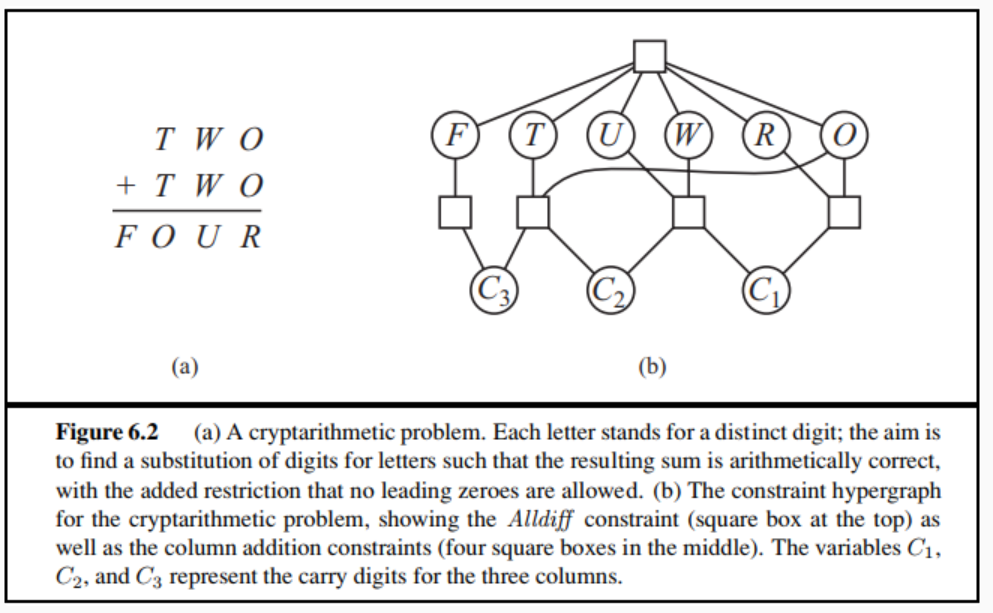
\includegraphics[width=\linewidth*2/3]{image/figure6.2.png}
\end{figure}

% domains
\noindent First of all, the \textbf{domains} are
\begin{itemize}
\item $C_1$: $\{1\}$
\item $C_2, C_3$: $\{0,1\}$
\item others: $\{0,1,2,3,4,5,6,7,8,9\}$
\end{itemize}
% constraints
And the \textbf{constraints} are as following:
\begin{itemize}
\item $F, T, U, W, R, O$ are different
\item $C_1=2\times O // 10$, $R=2\times O \% 10$, here "$//$" means an integer division with remainder, thus $C_1$ is an interger quotient.
\item $C_2=(2\times W + C_1) // 10$, $U=(2\times W + C_1) \% 10$
\item $C_3=(2\times T + C_2) // 10$, $O=(2\times T + C_2) \% 10$
\item $F=C_3$
\end{itemize}

\noindent \textbf{The 3 methods (forward checking, MRV, least-constraining-value(LCV)) are compatible, so I'll use them all.}

\begin{enumerate}[label={\arabic*. }]
\item choose $C_3$ (MRV); choose $1$ for $C_3$ (LCV); \\
domain of $F$ becomes $\{1\}$, \\
domain of $T$ becomes $\{5,6,7,8,9\}$
\item choose $F$ (MRV); choose $1$ for $F$ (only choice); \\
remove $1$ from domain of others due to alldiff
\item choose $C_2$ (MRV); choose $0$ for $C_2$ (LCV); \\
domain of $W$ becomes $\{0,2,3,4\}$, \\
domain of $O$ becomes $\{0,4,6,8\}$ (must be even)
\item choose $C_1$ (MRV); choose $0$ for $C_1$ (LCV); \\
domain of $O$ becomes $\{0,4\}$, \\
domain of $R$ becomes $\{0,8\}$, \\
domain of $U$ becomes $\{0,4,6,8\}$
\item choose $O$ (MRV); choose $4$ for $O$ (LCV); \\
domain of $R$ becomes $\{8\}$; \\
domain of $T$ becomes $\{7\}$
remove $4$ from domain of others due to alldiff
\item choose $R$ (MRV); choose $8$ for $R$ (only choice); \\
remove $8$ from domain of others due to alldiff
\item choose $T$ (MRV); choose $7$ for $T$ (only choice); \\
remove $7$ from domain of others due to alldiff
\item choose $U$ (MRV); choose $6$ for $U$ (forward checking). Otherwise, $U$ has to be 0, causing $W$ being 0, which is not allowed. \\
domain of $W$ becomes $\{3\}$
\item choose $W$ (MRV); choose $3$ for $W$ (only choice)
\end{enumerate}

\noindent After steps above, we find a \textbf{solution}:
$$F=1,T=7,O=4,U=6,W=3,R=8$$

\newpage
\section*{6.11}
\noindent \textbf{Use the AC-3 algorithm to show that arc consistency can detect the inconsistency of partial assignment $WA=green$, $V=red$ for the problem shown in Figure 6.1.}
\begin{figure}[H]
\centering
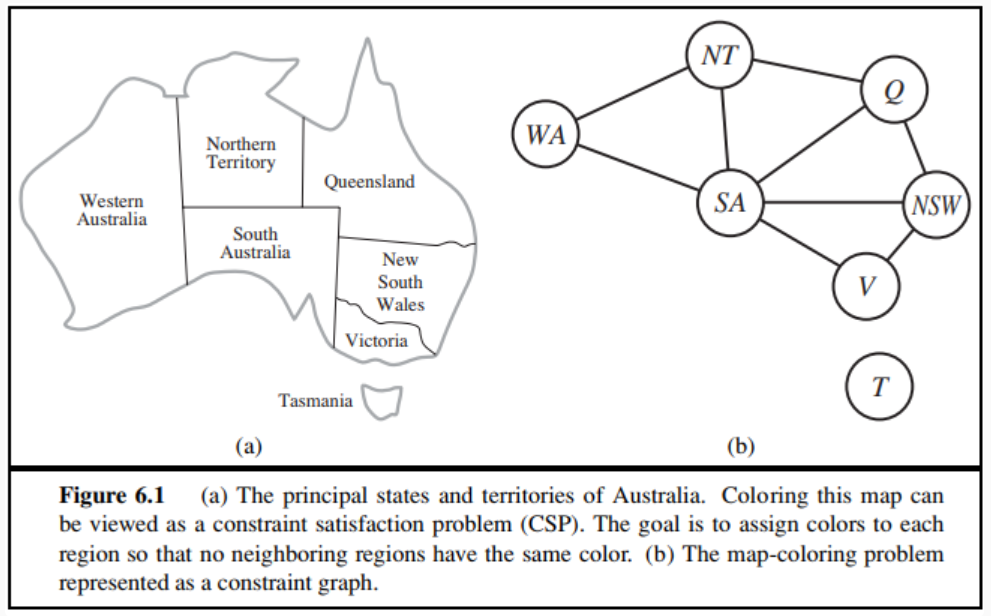
\includegraphics[width=\linewidth*2/3]{image/figure6.1.png}
\end{figure}

\noindent The steps of running AC-3 algorithm is as following:
\begin{enumerate}[label={\arabic*. }]
\item the queue contains all arcs: 
	\begin{align*}
	\{&(WA,NT), (WA,SA), (NT,Q),(NT,SA),(NT,WA), \\
	&(SA,WA),(SA,NT),(SA,Q),(SA,NSW),(SA,V),\\
	&(Q,NT),(Q,SA),(Q,NSW),\\
	&(NSW,Q),(NSW,SA),(NSW,V),(V,SA),(V,NSW)\}
	\end{align*}
\item after checking all elements above, the remaining legal assignments are: 
	\begin{center}
	\begin{tabular}{|c|c|c|c|c|c|c|}
	\hline
	WA & NT & SA & Q & NSW & V & T \\
	\hline
	$g\ \ $ & $r\ b$ & $\ \ b$ & $rgb$ & $\ gb$ & $r\ \ $ & $rgb$ \\
	\hline
	\end{tabular}
	\end{center}
	and then we still need to check:
	\begin{align*}
	\{&(NT,Q),(NT,SA),(NT,WA)\\
	&(SA,WA),(SA,NT),(SA,Q),(SA,NSW),(SA,V),\\
	&(NSW,Q),(NSW,SA),(NSW,V)\}
	\end{align*}
\item after checking all elements above, the remaining legal assignments are: 
	\begin{center}
	\begin{tabular}{|c|c|c|c|c|c|c|}
	\hline
	WA & NT & SA & Q & NSW & V & T \\
	\hline
	$g\ \ $ & $r\ b$ & $\ \ b$ & $r\ \ $ & $\ g\ $ & $r\ \ $ & $rgb$ \\
	\hline
	\end{tabular}
	\end{center}
	and then we still need to check:
	\begin{align*}
	\{&(Q,NT),(Q,SA),(Q,NSW),\\
	&(NSW,Q),(NSW,SA),(NSW,V)\}
	\end{align*}
\item after checking all elements above, the remaining legal assignments are: 
	\begin{center}
	\begin{tabular}{|c|c|c|c|c|c|c|}
	\hline
	WA & NT & SA & Q & NSW & V & T \\
	\hline
	$g\ \ $ & $\ \ b$ & $\ \ b$ & $r\ \ $ & $\ g\ $ & $r\ \ $ & $rgb$ \\
	\hline
	\end{tabular}
	\end{center}
	and then we still need to check:
	\begin{align*}
	\{&(NT,Q),(NT,SA),(NT,WA)\}
	\end{align*}
\item this time, $(NT,SA)$ will be inconsistent(both have the only choice of blue), thus we know AC-3 algorithm can detect the inconsitency of this circumstance.
\end{enumerate}

\vspace{5em}
\section*{6.12}
\noindent \textbf{What is the worst-case complexity of running AC-3 on a tree-structured CSP?}

\noindent Suppose that there are $E$ edges in this tree-structured CSP.\\
If nodes' domains are changed(can only be decreased) in each iteration of a whole queue(excluding newly added ones), then we need check $E$ more arcs per-iteration.\\
Thus, suppose $D$ is the largest domain size, then the worst-case complexity of running AC-3 on a tree-structured CSP is $O(ED)$


\end{document}




